% IEEE standard conference template; to be used with:
%   spconf.sty  - LaTeX style file, and
%   IEEEbib.bst - IEEE bibliography style file.
% --------------------------------------------------------------------------

\documentclass[letterpaper]{article}
\usepackage{spconf,amsmath,amssymb,graphicx,float,enumitem,url,algpseudocode}

% Example definitions.
% --------------------
% nice symbols for real and complex numbers
\newcommand{\R}[0]{\mathbb{R}}
\newcommand{\C}[0]{\mathbb{C}}

% bold paragraph titles
\newcommand{\mypar}[1]{{\bf #1.}}

% Title.
% ------
\title{Optimization and parallelization of diffusion solvers\\
using alternating direction implicit and random walk methods}
%
% Single address.
% ---------------
\name{Samuel Maloney} 
\address{Department of Mathematics\\ETH Z\"urich\\Z\"urich, Switzerland}

% For example:
% ------------
%\address{School\\
%		 Department\\
%		 Address}
%
% Two addresses (uncomment and modify for two-address case).
% ----------------------------------------------------------
%\twoauthors
%  {A. Author-one, B. Author-two\sthanks{Thanks to XYZ agency for funding.}}
%		 {School A-B\\
%		 Department A-B\\
%		 Address A-B}
%  {C. Author-three, D. Author-four\sthanks{The fourth author performed the work
%		 while at ...}}
%		 {School C-D\\
%		 Department C-D\\
%		 Address C-D}
%

\begin{document}
%\ninept
%
\maketitle
%


% ----------------------------------------------------------------------
\begin{abstract}
An optimized code for diffusion is presented. 
\end{abstract}


% ----------------------------------------------------------------------
\section{Background}\label{sec:background}

\mypar{Motivation} 
Diffusion is important because...

\mypar{Mathematical Formulation}
Diffusion stuff $T(x,y)$ and electrostatic potential $u(x,y)$ on a two-dimensional domain $\Omega$ with boundary $\partial \Omega = \Gamma_0 \cup \Gamma_1 \cup \Gamma_N$. The problem is defined by the two BVPs

\begin{equation}
\begin{aligned}
-\mathbf{\nabla} \cdot (\sigma(T(x,y)) \mathbf{\nabla} u(x,y)) &= 0 & \text{ \ in \ } & \Omega \text{,} \\
u(x,y) &= 1 & \text{ \ on \ } & \Gamma_1 \text{,} \\
u(x,y) &= 0 & \text{ \ on \ } & \Gamma_0 \text{,}  \\
\mathbf{\nabla} u(x,y) \cdot \mathbf{n}(x,y) &= 0 & \text{ \ on \ } & \Gamma_N \\
\end{aligned}
\label{u}
\end{equation}

\begin{center}
and
\end{center}

can be solved iterativly as follows.
\begin{enumerate}[noitemsep]
\item Start with an initial guess for the temperature in the domain, e.g., $\mathbf{T} \equiv 0$. 
\item Solve BVP \eqref{u} with FEM for $\mathbf{u}$ using $\mathbf{T}$ from the previous step.
\end{enumerate}


% ----------------------------------------------------------------------
\section{Baseline Implementation}\label{sec:baseline}

In this section, we provide an overview of the algorithm behind the matrix assembly and sparse solver parts of the algorithm. In addition, we perform a cost analysis.

\mypar{Matrix assembly}
The FEM procedure entails looping through all elements (triangles) in the mesh and calculating 3-by-3 elemental matrices. As an example, for BVP \eqref{u}, the nine entries of the elemental matrix $A^e$ are given by
\begin{equation*}
A_{ij}^e = \int_e \sigma(T(x,y)) \phi_i(x,y) \phi_j(x,y) dxdy \text{ \, \ } i,j=1,2,3 
\end{equation*}
where the $e$ under the integral denotes integration over the area of the element, and the
\begin{equation*}
\phi_i(x,y) = \left\{ \begin{array}{ll} 
				1-x-y & \textrm{if $i=1$} \\ 
				x     & \textrm{if $i=2$}   \\
				y     & \textrm{if $i=3$}
				\end{array} \right. 
\end{equation*}
are the so-called shape functions.
The full matrix $A$ is then obtained through
\begin{equation*}
A_{kl} = \sum_{e \in \text{sup}(k) \cap \text{sup}(l)} A_{ij}^e 
\text{ \, \ } i,j=1,2,3 \text{ \, \ } k,l=1,...,N
\end{equation*}
where $k$ (or $l$) is the global vertex number corresponding to the $i$ (or $j$) vertex in the elemental matrix. The notation $e \in \text{sup}(k)$ means elements $e$ which are supported by vertex $k$, i.e., vertex $k$ must be a vertex of element $e$.

For BVP \eqref{T}, one needs to calculate 2-by-2 (in addition to 3-by-3) elemental matrices due to the non-homogeneous Neumann boundary condition. Since the mathematics of FEM is beyond the scope of this paper, we omit giving further details.

Moreover, Dirichlet boundary conditions need to be applied, which is accomplished by directly altering the values of the relevant entries of the full $N$-by-$N$ matrix $A$.

\mypar{Sparse CG solver}
The algorithm behind the CG method for solving Eq. \eqref{matrix} based on an intial guess $\mathbf{x}$ for the solution is shown next
\begin{algorithmic}
\State $\mathbf{b}_0 = \mathbf{b}-A\mathbf{x}$
\State $\mathbf{p}   = \mathbf{b}_0$ 
\For {$k=0, ..., N-1$}
\State $\alpha = \frac{\mathbf{b}_k^T\mathbf{b}_k}{\mathbf{p}^T A \mathbf{p}} $
\State $\mathbf{x} = \mathbf{x} + \alpha \mathbf{p}$
\State $\mathbf{b}_{k+1} = \mathbf{b}_k - \alpha A \mathbf{p}$ 
\If {$||\mathbf{b_{k+1}}|| \leq \epsilon$} 
\State $\text{break}$ 
\EndIf
\State $\beta = \frac{\mathbf{b}_{k+1}^T \mathbf{b}_{k+1}}{\mathbf{b}_k^T\mathbf{b}_k}$
\State $\mathbf{p} = \mathbf{b}_{k+1} + \beta \mathbf{p}$
\EndFor
\end{algorithmic}
and gives the exact solution $\mathbf{x}$ within at most $N$ iterations. Note how the above procedure only relies on a matrix-vector product, vector dot products and vector additions.

\mypar{Cost Analysis}
We define the cost of the code as the number of floating point operations (FLOPs) including additions, multiplications, divisions, as well as square root and arctan evaluations, and integer to double casts. Moreover, the number of reads and writes in bytes was counted in order to quantify the operational intensity.

The matrix assembly complexity is roughly $O(N)$ as it loops once over all elements\footnote{The number of elements in linear FEM on a triangular mesh is roughly $2N$, where $N$ is the number of vertices in the mesh.}. 

The sparse CG method scales roughly as $O(N^2)$ because both the FLOPs per iteration and the number of iterations required for convergence scale proportionally to $N$.


% ----------------------------------------------------------------------
\section{Proposed Method}\label{sec:yourmethod}

In this section we explain the main optimizations that were undertaken.
We discuss the optimizations of the matrix assembly and the solver in separate subsections.

\subsection{Matrix assembly}\label{subsec:assembly}

We divide the optimizations in 4 sets called \textit{revisions}.

\mypar{Baseline implementation}
Our baseline implementation uses the Eigen library for the assembly of the matrix.
The boundary condition is applied after the assembly.

\mypar{Revision 1}
This revision consists mainly of removing Eigen and replacing its data structures with
C arrays (stored in the compressed sparse row (CSR) format).
A modified version of the C quicksort code found at \cite{quickSort} was used to implement the triplet-to-CSR storage format conversion.

\mypar{Revision 2}
In this revision we used precomputations and scalar replacements.
We also reduced the order of Gauss quadrature for evaluating integrals from 7-point quadrature to 3-point quadrature,
still achieving desired accuracy.
Removing unnecessary floating point operations reduced the FLOP count by a factor of 8. 
Finally, we inlined simple and frequently called functions.
These modifications moved us from the compute bound to the memory bound region,
according to our instrumentation infrastructure.

\mypar{Revision 3}
This revision was targeted at reducing the size of the working set by exploiting the symmetry of the problem and storing only the upper halves of the matrices.

\mypar{Revision 4}
The final revision involved applying the boundary condition during initial matrix assembly.

\subsection{Solver}\label{subsec:solver}

The solver optimizations can be similarly broken down into four revisions, independent of those for the assembly.

\mypar{Scalar 1st revision (baseline)}
This is a direct implentation of the CG algorithm, and uses a modified version of code from the course lectures \cite{SPMVM} for the CSR format sparse matrix vector multiplication (SPMVM).

\mypar{Scalar 2nd revision}
The first improvements were simple complexity optimizations. Specialized versions of the vector additiion (VADD) and SPMVM sub-functions were added that removed N adds from each call to VADD and also required one less call to VADD overall.

\mypar{AVX}
Vectorization of the VADD and vector dot-product (VDOT) sub-functions was done by leveraging Intel fused-multiply-add (FMA) and advanced vector extension (AVX) intrinsics. As explained later in the experimental results section, the SPMVM was not vectorized.

\mypar{AVX + ILP}
Additional accumulators were implemented in the VDOT sub-function to improve instruction level parallelism (ILP). On the Skylake architecture used for development and testing, an FMA operation has a latency of 4 cycles and a gap of 0.5 cycles, so $4/0.5=8$ independent accumulators were implemented to allow for full FMA utilization even in a no cache miss scenario.


% ----------------------------------------------------------------------
\section{Experimental Results}\label{sec:exp}

In this section the results of numerical benchmarks of the code at various stages are presented. Runtime, performance, and roofline analyses were performed where applicable.

\mypar{Experimental setup}
Data for the matrix assembly was collected on a single core from an Intel Skylake Core i7-6700HQ running at 2.6 GHz with turbo boost disabled on Ubuntu 16. It has 64 KB L1 cache split equally into two 32 KB data and instruction caches, 256 KB L2 cache, 6 MB L3 cache, and a 34.1 GB/s bandwidth to main memory. The GNU C Compiler v6.2.0 was used with "-O3 -mavx2 -mfma -march=skylake -DNDEBUG" flags. The Intel time stamp counter (TSC) was used for runtime measurements.

The inputs for the mesh assembly are the mesh data files for the FEM method domain discretization. We used meshes of various sizes, up to $7\cdot10^4$ vertices.

\subsection{ADI}\label{subsec:ADI_results}
Runtime experiments were conducted on the matrix assembly code in isolation from the rest of the algorithm. Performance measuremnts are not included for the assembly code as different revisions have significantly differing FLOP counts, rendering performance comparisons invalid.

\mypar{Results}
The runtime plots of various revisions of the matrix assembly (see \ref{subsec:assembly}) are shown in Fig. \ref{fig:runtime_assemby}. Each consecutive revision of the assembly resulted in a~speedup. The largest improvement, of 1.85X, comes from removing Eigen.
Revision 2 was also of great significance at 1.70X.
The overall speedup from baseline to our best code is 4.8X.

\begin{figure}\centering
  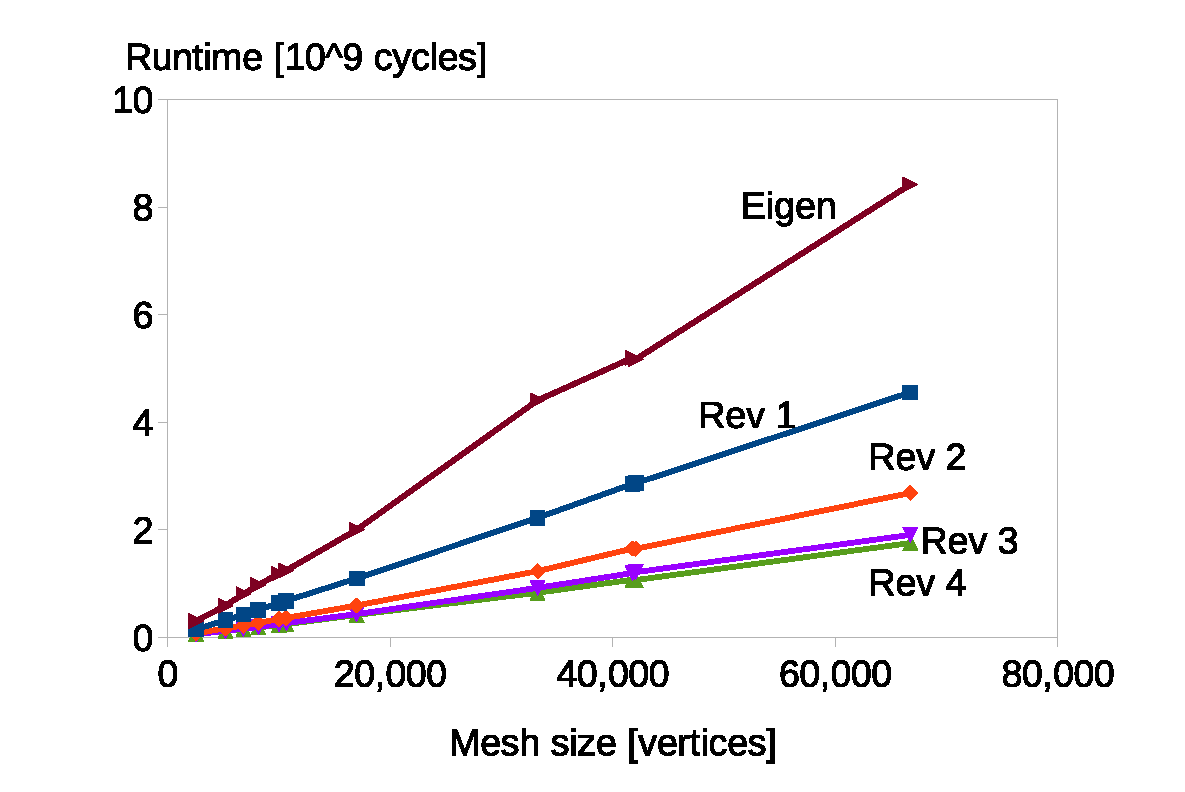
\includegraphics[width=\linewidth]{./plots/assembly_runtime.eps}
  \caption{Runtime analysis of the matrix assembly code.}
  \label{fig:runtime_assemby}
\end{figure}

\subsection{Solver}
Benchmarking experiments were conducted on the CG sparse linear system solver in isolation from the rest of the algorithm, as well as upon the individual sub-functions comprising the solver.

\mypar{Experimental setup} All data for the isolated solver benchmarks was collected in the CAB student labs. The processor used is a single core from an Intel Skylake Core i7-6700 running at 3.40 GHz with turbo boost and hyper-threading technologies disabled. It has 64 KB L1 cache split equally into two 32 KB data and instruction caches, 256 KB L2 cache, 8 MB L3 cache, and a 34.1 GB/s bandwidth to main memory. The GNU C Compiler v4.8.5 was used with "-std=c++11 -O3 -march=native -DNDEBUG -fno-tree-vectorize" flags. Linux perf, implemented using a C++ wrapper found online \cite{perfWrapper}, was used for cycle runtime and cache miss measurements.

For the tests on the VADD and VDOT sub-functions, arrays of pseudo-random numbers between 0 and 1 were used as inputs, with vector lengths ranging from $2^{11}$ to $2^{27}$ elements. For the SPMVM sub-function and full solver tests, the actual matrices generated in the assembly portion of the overall algorithm were piped to files for use in benchmarking, with the square matrix dimension ranging from 5193 to 66753. All experiments were performed with warm cache.

\mypar{Results}
Results of the roofline, performance, and runtime analyses of the CG solver will now be presented.

%\begin{figure}\centering
%  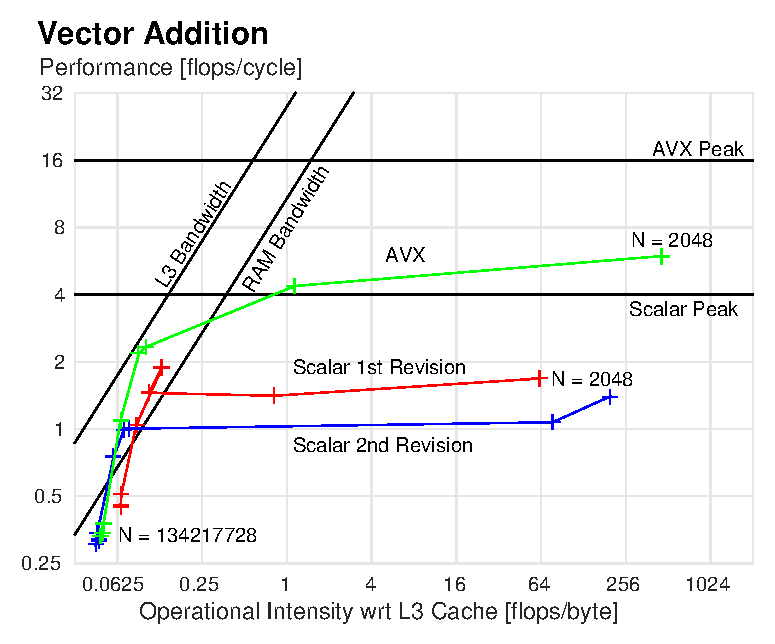
\includegraphics[scale=0.67]{./plots/roofline_vadd.eps}
%  \caption{Roofline analysis of the three implementations of the vector addition sub-function.\label{roofline_vadd}}
%\end{figure}
%
%In Fig.~\ref{roofline_vadd} a roofline analysis can be seen for the AVX and two scalar implementations of the VADD sub-function. For the 2nd scalar revision the decrease in performance with decreasing FLOP count indicates a memory-bound problem, particularly for large N, where the data points are seen to shift along the slope of the memory bandwidth. Utilizing AVX instructions increases performance more tightly to the memory bounds for large inputs and achieves the full 4X speedup for small inputs that benefit from caching.

\begin{figure}\centering
  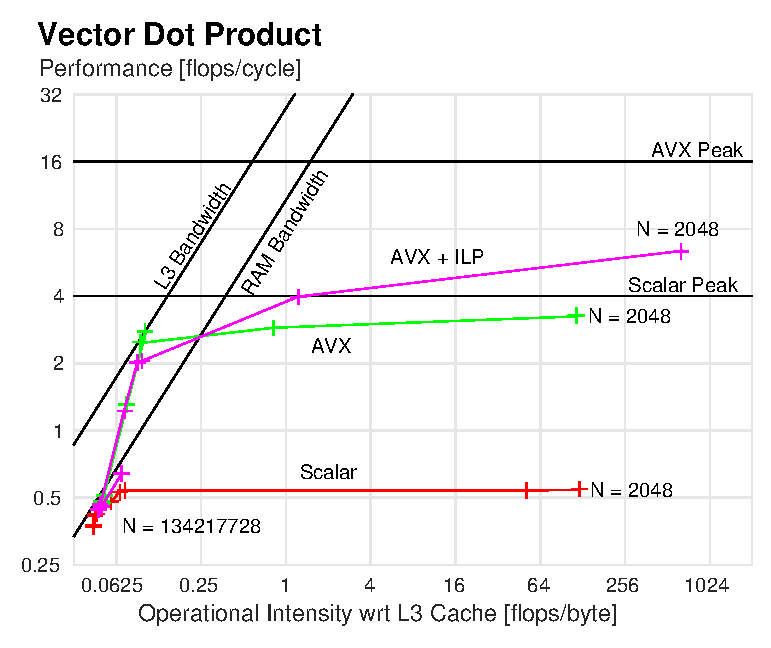
\includegraphics[scale=0.67]{./plots/roofline_vdot.eps}
  \caption{Roofline analysis of the three implementations of the vector dot product sub-function.\label{roofline_vdot}}
\end{figure}

A similar roofline analysis for the VDOT sub-function is seen in Fig.~\ref{roofline_vdot} where moving from scalar to AVX code pushes the performance tightly to the memory bounds for large inputs. For small inputs a speedup of $\approx$6X is observed, greater than the expected 4X, which is most likely due to the increase in ILP when moving to AVX, as the 4-element AVX vector essentially acts as four independent accumulators. This increased ILP is then fully exploited in the fastest version, giving total speedup of $\approx$12X for small inputs.

As mentioned previously, the AVX revision does not use a vectorized version of the SPMVM sub-function. A simple vectorization scheme was originally implemented, and while performance was measured to increase, runtime measurements proved slower for all input sizes. This is most likely due to the extreme sparsity of our matrices ($\geq$99.9\%) which makes the overhead of reducing the AVX vector at the end of each row outweigh any gains, producing only spurious performance gain and increasing runtime.

Fig.~\ref{perf_solver} shows a performance comparison of the latter three revisions of the complete CG solver (the 1st scalar revision is omitted as it has a different FLOP count). We can see that large gains of almost 2X for the AVX revision and 4X for the fastest AVX + ILP revision are observed for the smallest inputs, and possibly larger increases might have been observed if smaller inputs had been available. However, for most larger inputs increases of performance of only around 40\% are achieved, owing to the strong memory constraints of solving such a sparse linear system.

\begin{figure}[H]\centering
  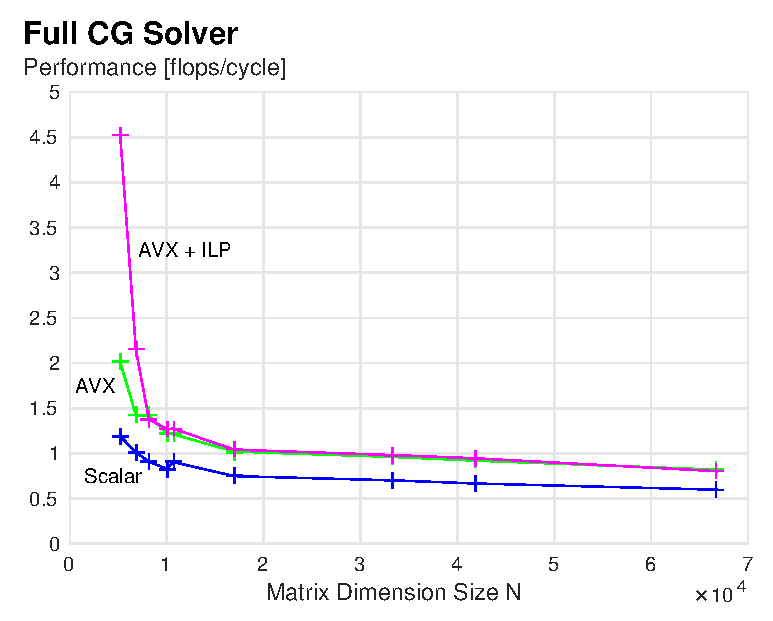
\includegraphics[scale=0.67]{./plots/perf_solver.eps}
  \caption{Performance analysis of three implementations of the
  conjugate gradient solver. Only the 2nd scalar revision is shown, such that all FLOP counts are roughly the same.\label{perf_solver}}
\end{figure}

\begin{figure}\centering
  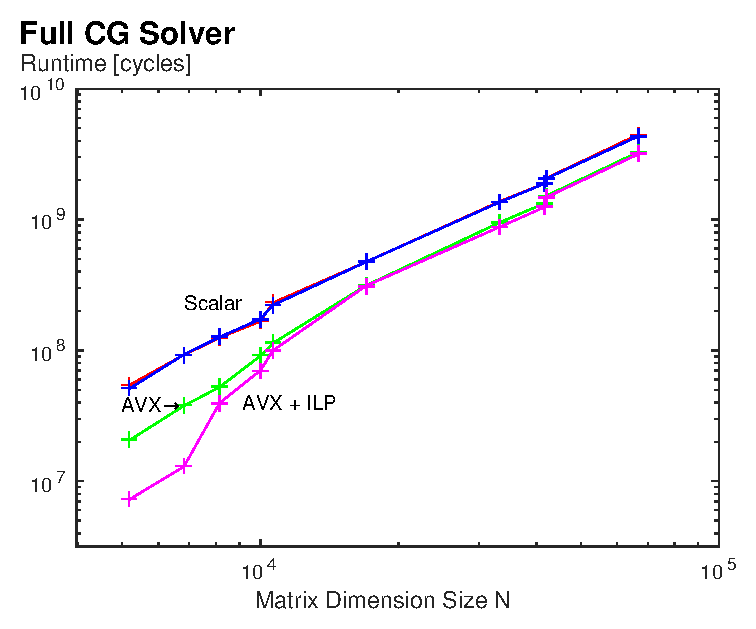
\includegraphics[scale=0.67]{./plots/runtime_solver.eps}
  \caption{Runtime analysis of the four implementations of the
  conjugate gradient solver. Note that both scalar revisions are shown, but are almost entirely overlapping in the plot.\label{runtime_solver}}
\end{figure}

Runtime data for the four revisions of the CG solver is presented in Fig.~\ref{runtime_solver}. As in the performance case, the most significant runtime decreases, by factors of 2.6X and 7.5X for the AVX and AVX + ILP revisions respectively, are seen for the smallest inputs. For larger inputs, the factor shrinks to 1.4X - 1.5X for both vectorized revisions. It is also seen that the two scalar revisions show negligible difference in runtime despite the decrease in flop count for the 2nd revision, confirming the memory bound nature of the problem. 

\begin{figure}\centering
  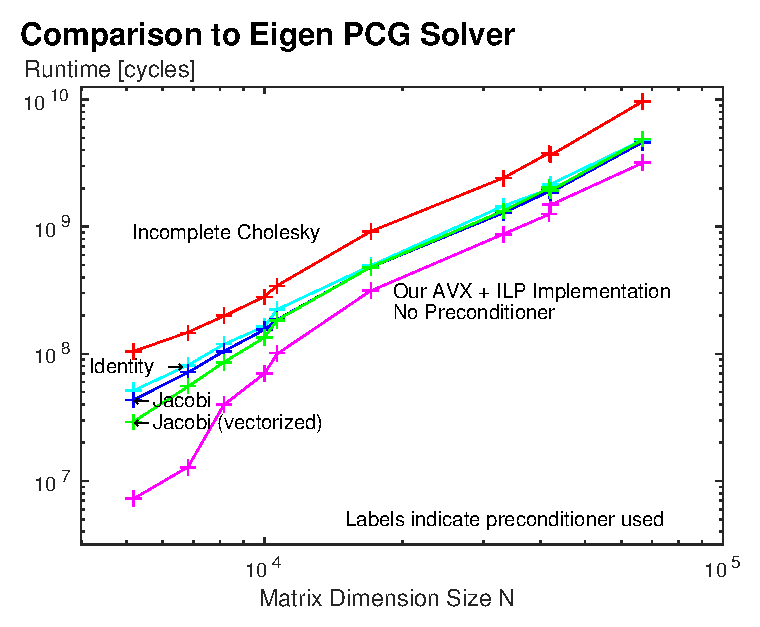
\includegraphics[scale=0.67]{./plots/runtime_vs_Eigen.eps}
  \caption{Runtime comparison of our fastest implementation vs the Eigen template library preconditioned CG (PCG) solver using various preconditioners.\label{runtime_vs_Eigen}}
\end{figure}

Finally, in Fig.~\ref{runtime_vs_Eigen} is presented a runtime comparison of our best revision against the Eigen template library with the same convergence criteria. It must be noted that Eigen (and most similar libraries) only provides a \emph{preconditioned} CG solver. Thus, while the comparison includes a test using Eigen's identity preconditioner, which renders the algorithms mathematically identical, there is no guarantee that Eigen does not still incur some unaccounted for overhead if it has no specialized implementation. However, as no unconditioned CG solvers in fast libraries were readily available, this was deemed a suitably reasonable approximation for comparison. For the sake of completeness all of the preconditioners available from Eigen were tested, and for the best-performing Jacobi preconditioner a test without using the -fno-tree-vectorize compiler flag was conducted to see if the difference was due to reliance by Eigen on compiler vectorization. While this resulted in Eigen's best runtime, our implementation is still quicker for all input sizes.

%\begin{figure}\centering
%  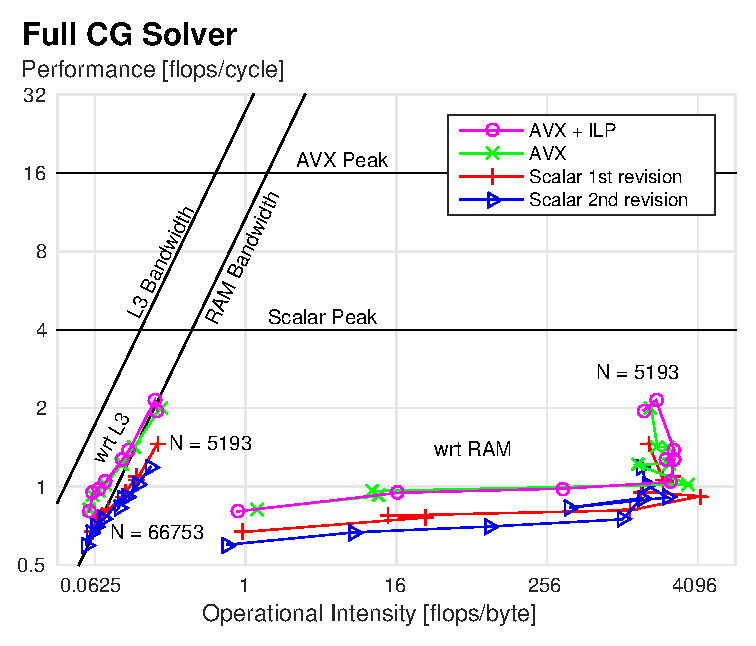
\includegraphics[scale=0.67]{./plots/roofline_solver.eps}
%  \caption{Roofline plot of four implementations of the conjugate gradient solver.\label{roofline_solver}}
%\end{figure}

\subsection{Total runtime}
For measuring the effect of progressive optimizations on runtime, we used revision 1 of the matrix assembly together with the 2nd scalar revision of the CG solver and revisions 2-4 of the assembly paired with the symmetric AVX + ILP revision of the CG solver.
The baseline 'Eigen' revision uses Eigen's sparse LU solver becuase the original naive implementation of the Dirichlet boundary conditions destroyed the natural symmetry of the system and thus precluded the use of a CG solver, which is only guaranteed to converge for a symmetric positive definite (SPD) matrix. FEM systems are naturally SPD, and ensuring this property was preserved in later revisions was itself an algorithmic optimization to allow the use of a faster symmetric solver.
The runtime plot is shown in Fig. \ref{fig:runtime_total}, using the same inputs and experimental setup as for the matrix assembly measurements (see \ref{subsec:assembly_results}). Consecutive improvements in the runtime are visible, with a cumulative speedup by a factor of 2.4X observed.
\begin{figure}[H]\centering
  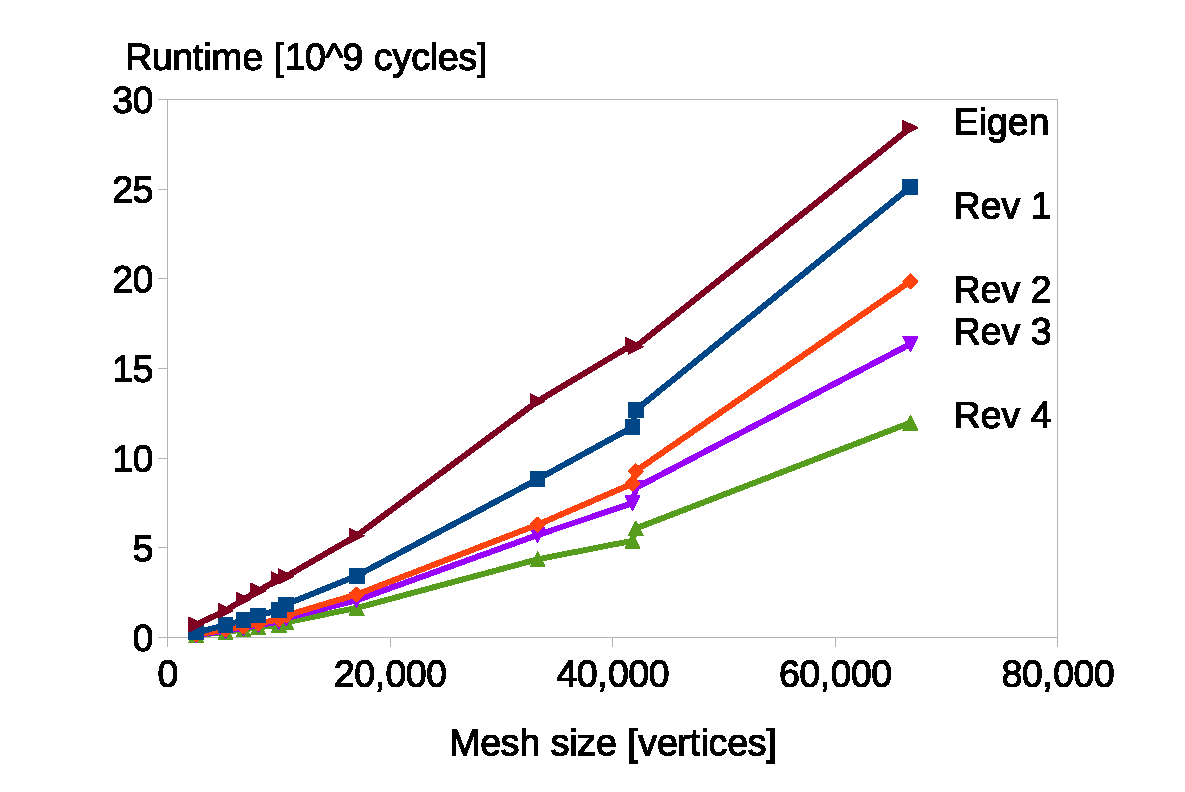
\includegraphics[width=\linewidth]{./plots/total_runtime.eps}
  \caption{Runtime analysis of the complete algorithm.}
  \label{fig:runtime_total}
\end{figure}


% ----------------------------------------------------------------------
\section{Conclusion}
Conclude things

% ----------------------------------------------------------------------


\begin{thebibliography}{99}

\urlstyle{same}

\bibitem{transpose}{user2927848. (2016, Mar 23). \emph{m256d TRANSPOSE4 Equivalent} [Online]. Available: \url{https://stackoverflow.com/questions/36167517/m256d-transpose4-equivalent}}

\end{thebibliography}

\end{document}
